\documentclass[a4paper,11pt]{article}
\usepackage[spanish]{babel}
\usepackage{
			ucs
			,amsfonts
			,amssymb
			,acronym
			,verbatim
			,rotating
			,graphicx
			,enumerate
			,fancyhdr
            ,mathrsfs
            ,array
			}

\usepackage{tikz}
\usetikzlibrary{shapes,arrows}

\pagestyle{fancy}
\addtolength{\textheight}{1.0in}
\addtolength{\textwidth}{0.5in}
\addtolength{\voffset}{-1.0in}


\fancyhf{}
\fancyhead[L]{{\bfseries Algoritmos y Estructuras de Datos. Pr\'actica 1 \hfill Diagramas de Flujo - Resoluci\'on}}
\fancyfoot[LE,RO]{\thepage}

\fancypagestyle{firstpage}{
\fancyhf{}

\fancyhead[L]{
\small{UNaB. Universidad Nacional Almirante Brown.} \\
{\bfseries Algoritmos y Estructuras de Datos. Pr\'actica 1 \hfill \\ Diagramas de Flujo - Resoluci\'on}}
\fancyfoot[LE,RO]{\thepage}
}

\thispagestyle{firstpage}

\begin{document}
 
 ~ \\   

Soluciones a algunos de los problemas planteados en la Pr\'actica 1. 

\begin{enumerate}

\item Ejercicio \emph{1-a}. Subir en ascensor a piso $X$.

\begin{figure}[h]
\centerline{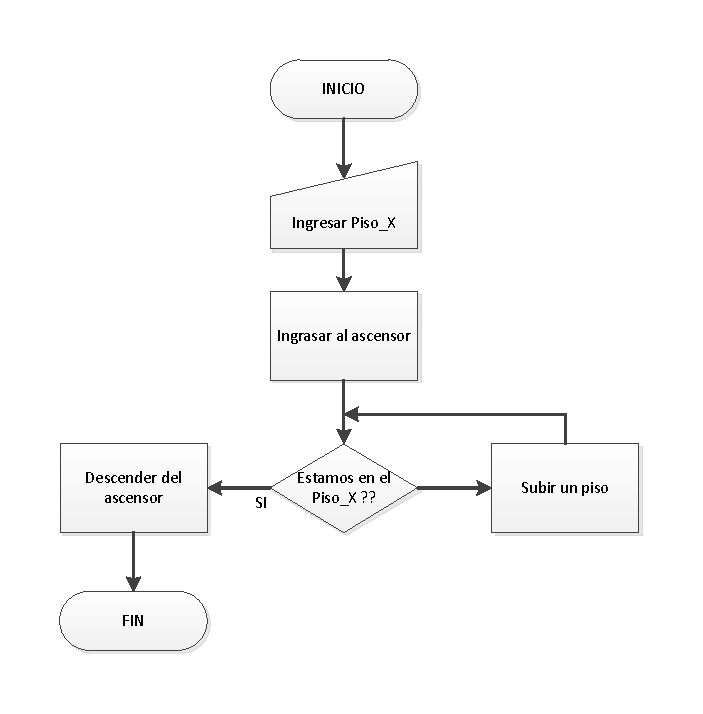
\includegraphics[height=7in]{Ejer_1a.pdf}}
\end{figure}

\newpage

\item Ejercicio \emph{2-a}. Calcular el promedio de tres n\'umeros utilizando una calculadora.

\begin{figure}[h]
\centerline{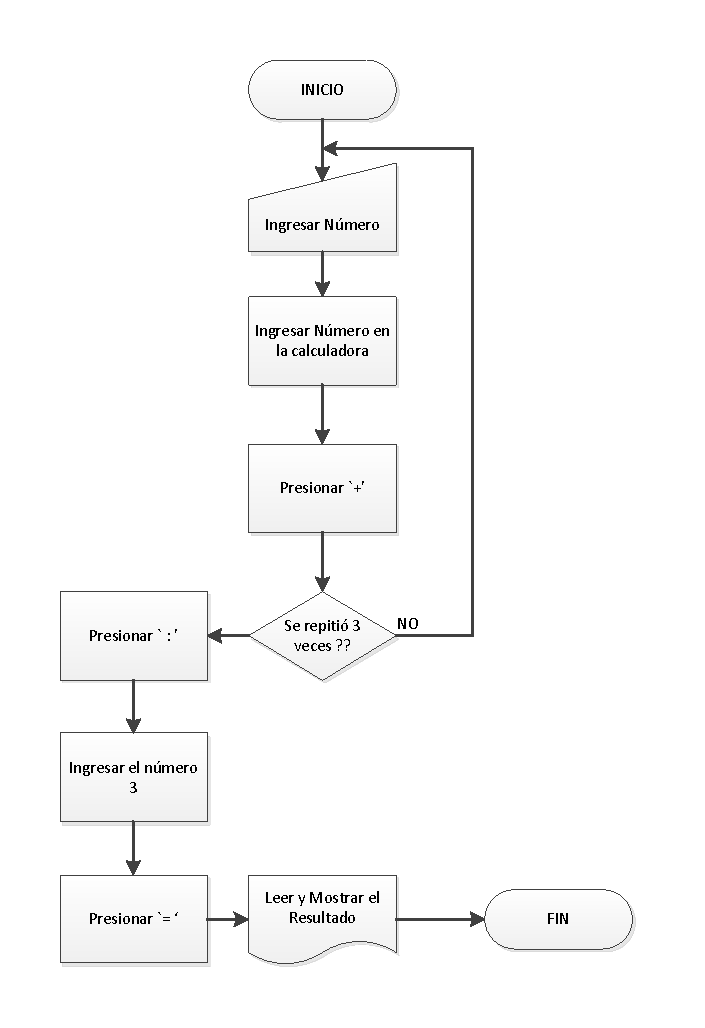
\includegraphics[height=7in]{Ejer_2a.pdf}}
\end{figure}

\newpage 

\item Ejercicio \emph{2-d}. Separar un mazo de naipes en cuatro pilas, una para cada palo.

\begin{figure}[h]
\centerline{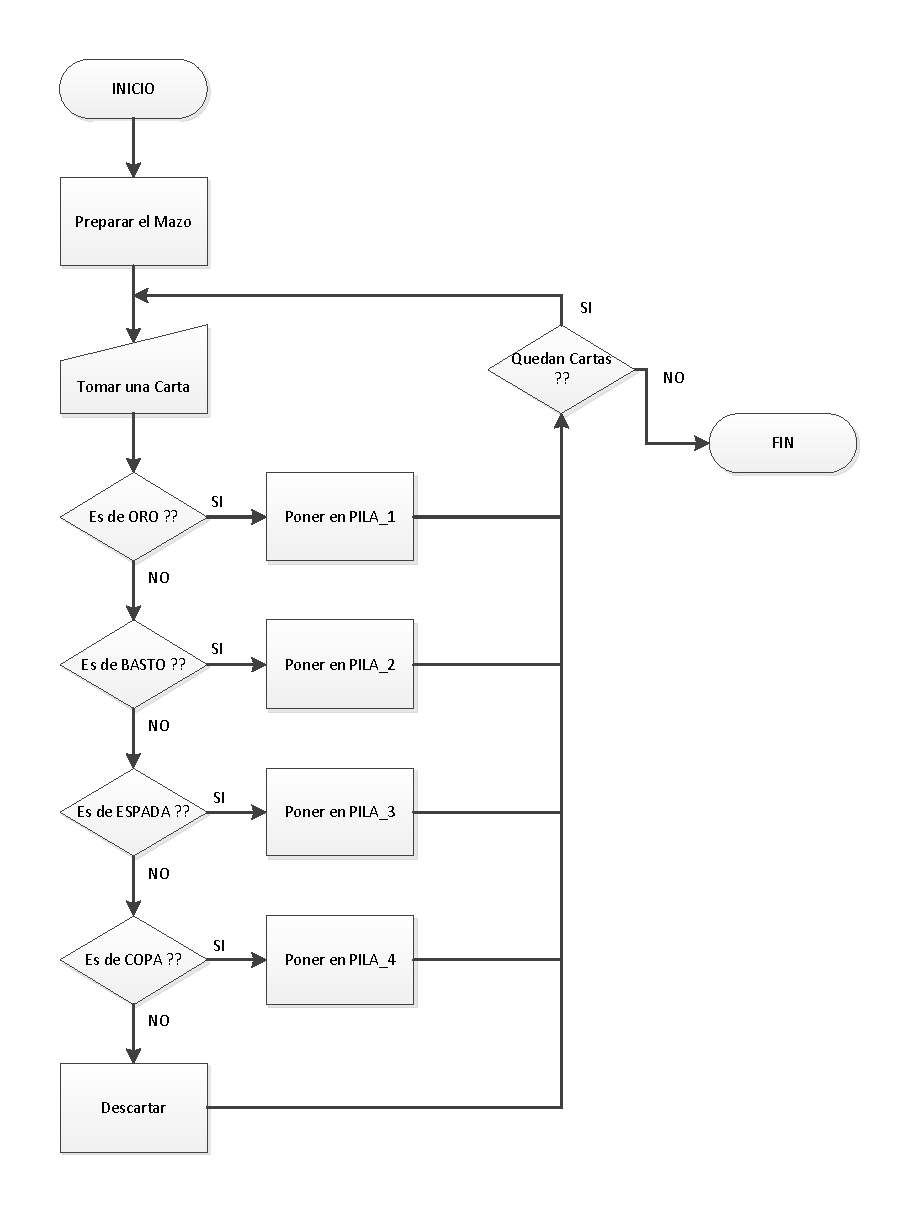
\includegraphics[height=5.5in]{Ejer_2d.pdf}}
\end{figure}

\newpage

\item Ejercicio \emph{3-b}. De una pila de tarjetas numeradas informar cu\'al es la mayor.

\begin{figure}[h]
\centerline{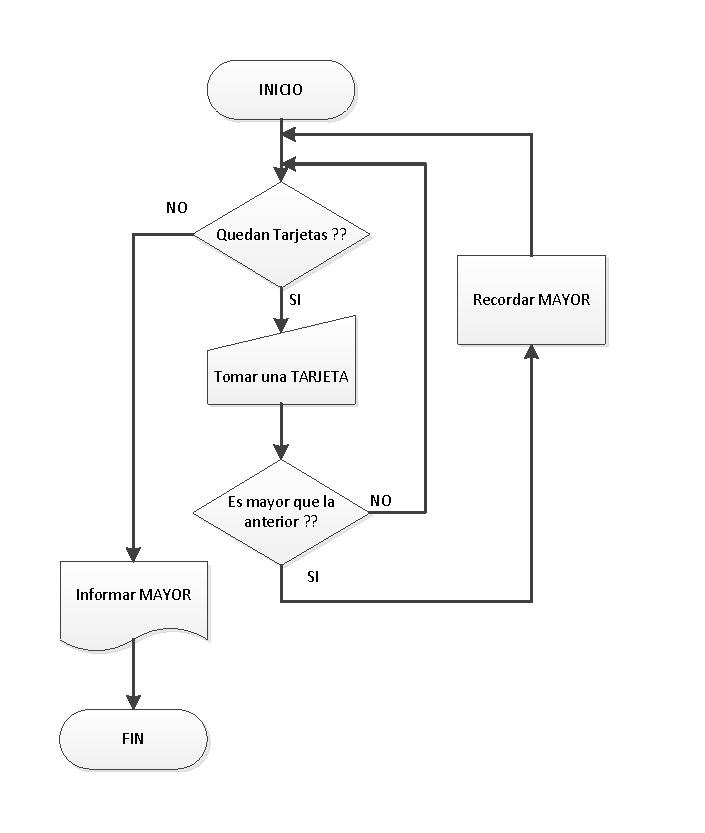
\includegraphics[height=7in]{Ejer_3b.pdf}}
\end{figure}

\newpage

\item Ejercicio \emph{4-b}. Dada una pila de $N$ naipes, obtener la suma (cada naipe vale su n\'umero).

\begin{figure}[h]
\centerline{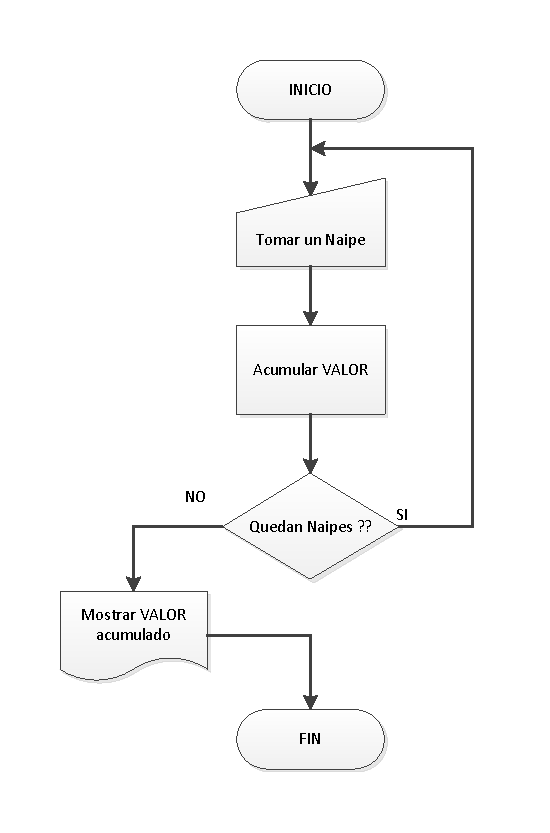
\includegraphics[height=7in]{Ejer_4d.pdf}}
\end{figure}

\newpage

\item Ejercicio \emph{6}. Dise\~nar un algoritmo que calcule el promedio de una serie de n\'umeros positivos entrados por teclado. El ingreso del valor igual a 0 indicar\'a el final del ingreso de datos.  
    
\begin{figure}[h]
\centerline{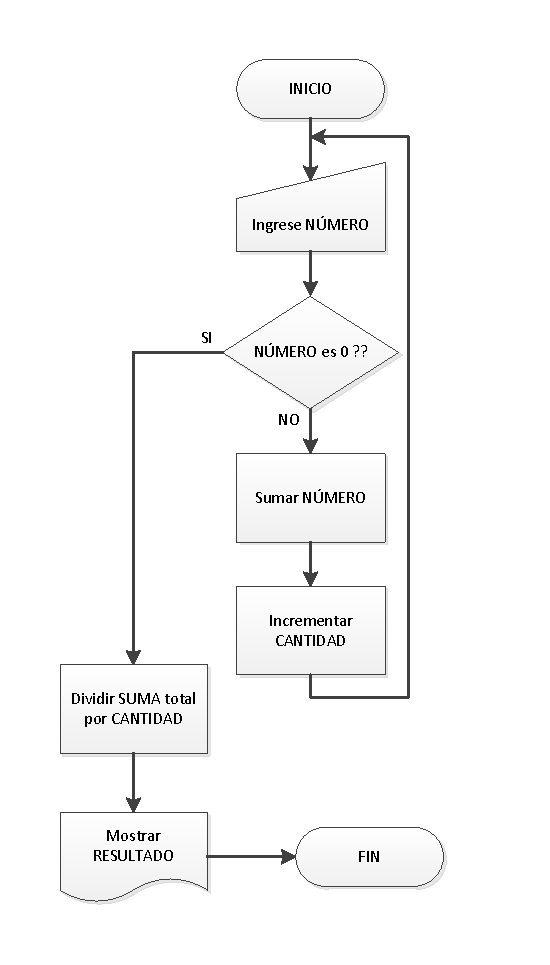
\includegraphics[height=7in]{Ejer_6.pdf}}
\end{figure}

\newpage

\item Ejercicio \emph{9}. Dise\~nar el algoritmo que permita dado tres n\'umeros, determinar si la suma de cualquier pareja de ellos es igual al tercer n\'umero. Si se cumple esta condici\'on deber\'a imprimir la palabra ``iguales'' sino ``distintos''.
    
    \begin{figure}[h]
\centerline{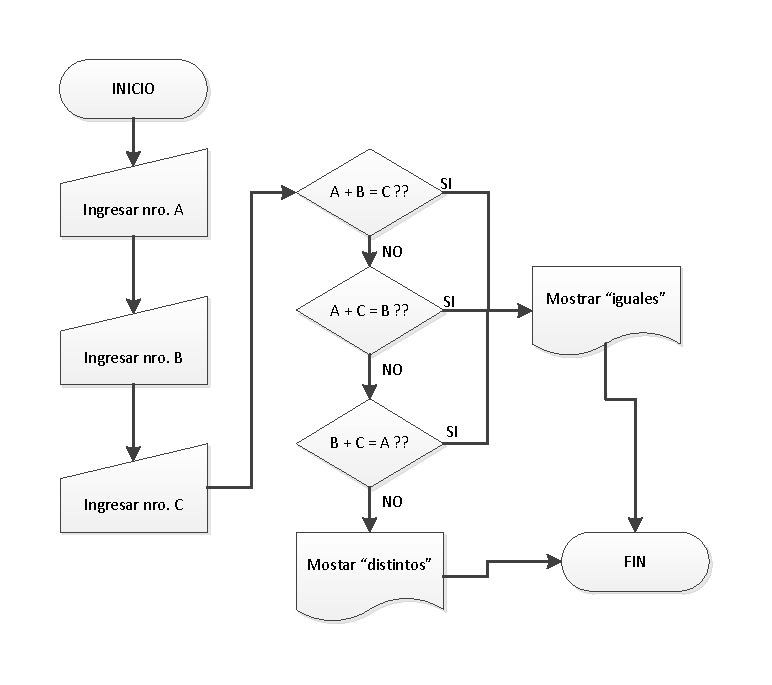
\includegraphics[height=7in]{Ejer_9.pdf}}
\end{figure}

\end{enumerate}
\end{document}
